






\subsection{image captioning}

Image captioning is an extensively researched field where visual-grounding is at the  center of its focus. The methods of image captioning provide insights helpful for tasks that combine vision an language. In this section we review two main methods used in image captioning,feature extraction and attention mechanisms.   

Video \cite{Lin2014VisualSS}


\subsubsection{Feature extraction-CNN+RNN}

Feature extraction methods can be divided into two main groups. The first group relies on statistical language models(described in the previous section as transparent function). The second group relies on encoder-decoder neural network model that deep extracts features.\cite{Imagecap}

\paragraph{Encoder-Decoder(CNN-RNN)}



Convulutional neural networks are at the core of feature extraction methods. CNN applications, nonetheless, take a vital role in many computer vision tasks. We see CNN and its modified models (such as recurrent-CNN) used in tasks as object recognition \cite{liang2015recurrent} \cite{objdet} \cite{Ren2015FasterRT} , image classification \cite{simonyan2014very} \cite{imclassfication},and  semantic segmentation \cite{hariharan2015hypercolumns} \cite{imseg}. 

The reason for using CNN for image processing  is its ability to reduce the high dimensionality of images. Image features contain large sizes represented in pixels which would require large number of parameters to train. CNN reduces the dimensions of an image by learning how to process a matrix from a large window such as 250x250 pixels into a smaller one as 25x25. Through computing the convolution values of the image matrices and executing pooling computations, this process reduces the image into a smaller representation. The latter reduces the computational load and helps in processing and classifying the images faster.   


The encoder-decoder caption generation has a CNN encoder and an RNN decoder.\cite{vinyals2015tell} is an example of an end-to-end neural captioon generation model. In the neural model the CNN process the image features, and the last hidden layer passed to an RNN to generate a description. This method is a sequence modeling that is similar to machine translation. This means that image features are translated into words. The sequence is predicted by finding the probability of a certain description from a corpora given the features of an image. 

RNN are known to be used widely in language technology applications. Rnn is used , for example in  text-to-speech \cite{arik2017deep} and  machine-translation \cite{cho2014learning},\cite{Wu2016GooglesNM}. The advantage that the RNN gives to these tasks is that the output size is not fixed and that each output depends on the previous one. Such an incremental-sequence prediction is suitable for sentence predictions in respect to word dependency.  

RNNs have a issue of vanishing gradient-descent. The gradient descent is an optimization algorithm that minimizes the error calculated in the loss function. Optimization, in brief description, is important for the learning process. It updates the model's parameters which determines the  direction taken in the next time-step. This information is calculated given the input-output and the values of the parameters from the previous time-stamps. The gradients is reduced at every step due the value deductions in the activation function. When the gradient is reduced to almost zero value, it will be updating the parameters with no useful values, and therefore, learning seizes to improve. 

Long-Short-Memory network (LSTM)  provides a good alternative for avoiding the disappearing gradient. The gradient in RNNS vanishes in long sequences where the gradient keeps reducing. The architecture of the LSTM allows it to keep information stored for very long sequences. The latter gives it the ability to control the values of the gradient by updating it with information stored in the 'forget gate' form previous steps, preventing the gradient from vanishing.  



\paragraph{Feature extraction- statistical language model}

Statistical language model, as in \cite{fang2015captions}, generate descriptions in three stages. First it detects words in an image using a convolutional neural network (CNN) for extracting image features. The incorporation of language at this stage happens using multi-instance learning(MIT)\cite{zhang2005multiple}. The second stage, the statistical language model detects the most likely sentence to make of the words from a pre-defined corpus. In the third stage the sentences undergoes a re-ranking stage where the sentences are combined to generate captions. 


\paragraph{Attention-mechanisms}


In the previous section the discussion on the methods and implementation 

\subsection{Dialogue and VQA}

In this section of the text we discuss the capabilities of computers to exhibit more intelligent behaviour. Image-captioning and its methods showed an insight to how much computers could see and understand what its seeing. However, acquiring language in the visual world would require computers to be able to communicate what it sees. Otherwise, in order to say that a computer is visually or linguistically intelligent one should imagine the computer having to pass the Turing test in a visual surrounding. 

Researchers attempt to improve systems that are capable to hold a dialogue with a visual content.\cite{das2017visual} trains a system in  encoder-decoder model on a data set of 2 pairs dialogue with an image content.\cite{Skoaj2011ASF} trains a system on learning concepts with visual content in an interactive-learning approach. 

To make a true statement about the computer's capability to engage in a visual dialogue, it must be first ensured that the computer actually understands the questions being asked to it. Otherwise, dialogue is very complex with many elements determining it succession. In a dialogue with visual content, the computer must, furthermore, understand the questions within their visual context. It is reasonable that we see increasing research on "Visual Question Answering" and less on visual dialogue as a whole. Improvements in VQA intuitively means that we are moving closer in the direction of having an interaction with a computer in a visual dialogue.  


 \cite{VQA} is the first notable data-set published for Visual Question answering (VQA). The data-set consist of open-ended and free-form questions. The data contains 250,207 images from MS COCO \cite{lin2015microsoft} and other abstract scenes.The question types in the dataset require a range of different capabilities such as common-sense reasoning, knowledge-based reasoning, object-detection and active recognition.
 
 Data-sets that use MS COCO scenes such as \cite{gao2015talking}, \cite{yu2015visual} in addition to \cite{VQA} used human workers to write the texts for the scenes. Other data-sets are generated automatically such as \cite{ren2015exploring}. 


\cite{zhu2016visual7w} introduces a  unique QA data-set. The Visual7W consist of questions about an image with objects marked with regions in the image. Object grounding with image region introduced in \cite{krishna2016visual} contains the largest data-set with regions for both VQA and Image-captioning. Object-region approach is intended to improve visual grounding, by marking the regions of the image that the strings refer to.

restricted visual Turing test to evaluate visual understanding. The DAQUAR dataset is the first toy-sized QA benchmark built upon indoor scene RGB-D images. Most of the

\subsection{Embodied Question Answering}

\begin{figure}[H]
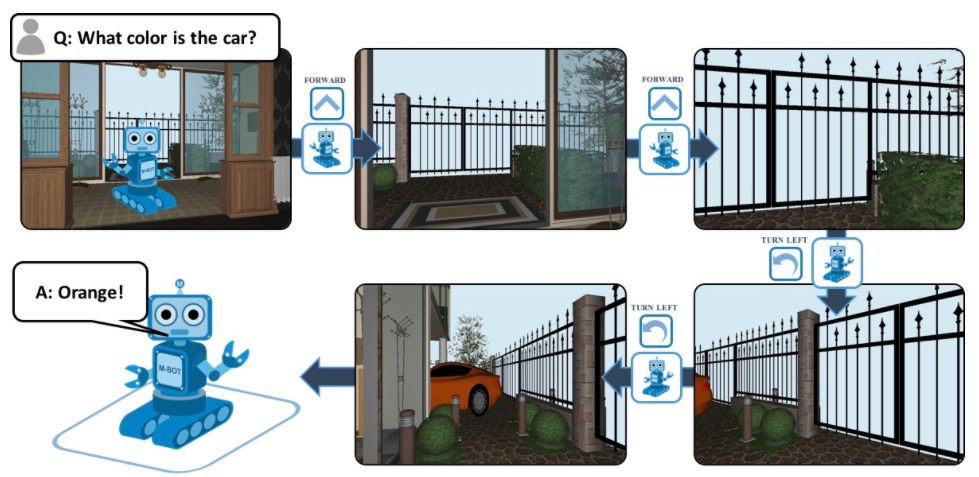
\includegraphics[scale=0.4]{latex/images/EmbodiedQuestionAnswering.png}
\label{fig:EQA}
\caption{The Robot is asked a question at a start position. It needs to look a round, collect information and decide on the next step to take. When it recognizes the car it stops and processes the scene to answer the question }
\end{figure}. 

Embodied Question Answering is a new interactive task presented as one of the tasks within the Habitat Platform\cite{embodiedqa}. The idea of the task is to allocate an agent at a random position in an  3D environment and ask it a question. To answer the question, the agent must intelligently explore the environment, collect information, and successfully navigate to the entity in question. EQA system navigates based on common reasoning, through an egocentric view, more or less imitating humans, it should be able to answer itself the common questions of “where am I?”, “where to go next?” and if asked a question about the car, as seen in \ref{fig:EQA}, it should be able to reason that cars are usually situated outside or in the garage and look for the exit. Once it navigates successfully to a point where it recognizes the car, the robot should stop and answer the question.  


\begin{figure}[H]
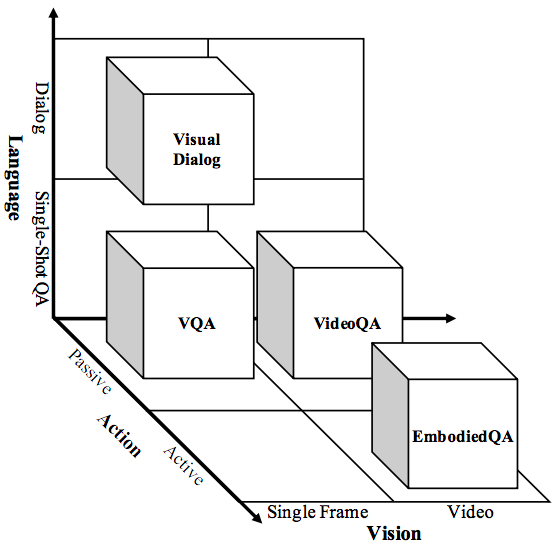
\includegraphics[scale=0.3]{images/Vision-language.png}
\caption{EQA in relation to other multi-modalitied  }
\ref{fig:multimodal}
\end{figure}.


 EQA shares some common ground with other multi-modality tasks of vision and language but is distinguished by other functionality. In figure \ref{fig:multimodal}  (paragraph to be written)



The novelty of this system is that it presumably solves a problem of navigating and performing tasks in unseen environments. Many of the earlier studies that deal with navigation such as \cite{kruijff2007situated}\cite{lauria2001training} require the system to have a localized map of the environment in order to be able to navigate in it. The problem of localization in robotic navigation is known as Simultaneous Localization and Map Building(SLAM). SLAM is a problem where a robot should be able to  map an unknown environment without a GPS or local map. Simultaneous localization is when a robot discover its surrounding and simultaneously construct a map while aware of its changing location. This means that the robot should extract information from its surrounding and learn the map as it goes \cite{grisetti2010tutorial} \cite{938381} \cite{8482266}. 



The answering system in the robot consist of two components. The first is navigation, and the second is Visual Question Answering. The navigator is responsible for navigating to the scene ... The agent needs to successfully navigate to the target object. Once the agent reaches the goal it would stop at the target location and would process the question and the visual input to answer the question.




In order to implement the whole embodied question answering we can say that the system consists of multiple combined parts, such as vision, navigation, reasoning and answering. However,the design of the system allows it to exclusively perform visual question answering on the baselines, without training and testing the navigation. The evaluation is done on the model that is responsible for question-answering at the scene point where the target object exists.Therefore, before discussing any other related constructs in the Habitat platform, such as agent, working flow, it is important to first look at the part of the system that this paper aims to evaluate. 









\subsubsection{navigation}



Habitat's navigation is referred to as PACMAN. It consist of two core components, planner and controller. The planner takes inputs from the vision and language model, and the encoding of hidden-layer and action of the previous time-step , then outputs action-decision. 

\begin{figure}[H]
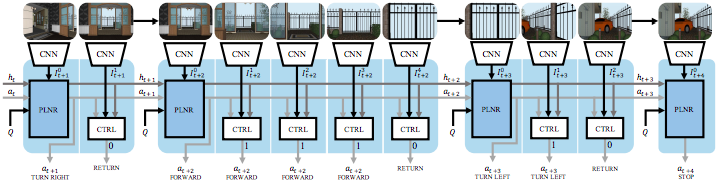
\includegraphics[scale=0.53]{images/nav.png}
\caption{}
\label{fig:nav}
\end{figure}

The controller takes the previous hidden state and action-decision and executes the action. As seen in \ref{fig:nav}, visual input is passed to the control then the controller classify the next decision of two possible decisions. Either to repeat the last action given by the planner or to return to the planner. The controller can repeat the same action maximum five times then it automatically returns to the planner. 

Visualization of the navigation is in figure (1). T stands for the planner's time-steps, t = 1,2,3...., and N(t),  n = 0,1,2,3.. denotes the controllers time-steps. The denotations of symbols explained clearer in the quotation : 


"\begin{math}  I_{t}^{n} \end{math}denote the encoding of the observed image at t-th planner-time and n-th controller-time. The planner is instantiated as an LSTM. Thus, it maintains a hidden state \begin{math} h^{t}\end{math}
(updated only at planner timesteps), and samples action 
\begin{math}  a_{t} \ \in \ \{forward,\ turn-left,\ turn-right,\ stop\} \end{math} "p(6)
\vspace{0.3cm}

For eample the first  step-decesion from the planner is denoted as such: 
\vspace{0.3cm}

\hspace{1cm}        \begin{math} a_{t} ,h_{t}{}\leftarrow PLNR\left( h_{t-1} ,I_{t}^{o} ,Q,a_{t-1}\right) \end{math},
        
\vspace{0.3cm}

The planner computes the next step-action  \begin{math} a_{t+1} \end{math} from input of the previous hidden layer \begin{math} (h_{t-1}) \end{math}, question encoding (Q), the previous action  \begin{math} a_{t-1} \end{math}, and the image input given to the PlNR \begin{math} (tI_{t}^{o}) \end{math}.The planner selects the action \begin{math} a_{t+1}\end{math} and update the hidden state \begin{math} h_{t+1} \end{math} then passes the control to the controller. 

\vspace{0.3cm}
(The basis of the controller decision is a bit unclear)

The controller decides to either repeat the action or return control to the planner. The controller's classification is based on the current hidden-state\begin{math} h_{t}  \end{math} and current action \begin{math} a_{t} \end{math} and the image observation from the planner + the image given at the controller's time-step. The denotation of the classification is as such: 

\vspace{0.3cm}

\[ \{0,1\} \ \backepsilon \ c_{n}^{t} \ \leftarrow CTRL\ \left( h_{t} ,a_{t} ,I_{t}^{n}\right)  \]

"if \begin{math} c_{n}^{t} = 1 \end{math} then the action \begin{math} a_{t} \end{math} repeats. Else \begin{math} c_{n}^{t} = 0 \end{math} or a max of 5 controller-times been reached, control is returned to the planner"p(6). The \begin{math} h_{t} \end{math}   \begin{math} a_{t} \end{math} coming from the planner act as an intent. The controller, initiated  as "feed-forward multi-layer perceptron with 1 hidden layer",repeats and controls the action in order to align \begin{math}  I_{t}^{n} \end{math} with intent given by the planner. 

\subsubsection{VQA Model}

\begin{figure}[H]
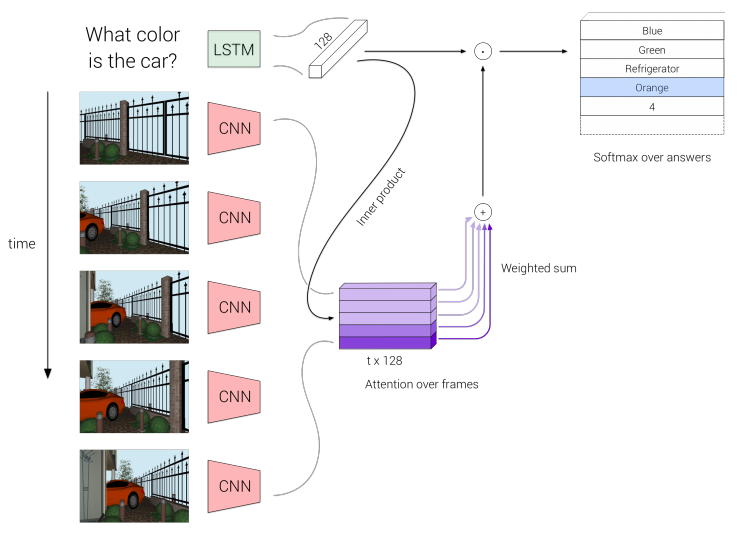
\includegraphics[scale=0.35]{latex/images/VQA.png}
\caption{}
\label{fig:VQ}
\end{figure}

(Text already exist .... To be completed)

The VQA model consists of two parts, one is a CNN model to extract features from the scene images(5 frames), and the other takes the question input and combine it with the wights of the images. Figure 1 illustrates the combination of the two parts. 





\subsection{Problem}



In an experiment we conducted on the VQA model, we noticed that the system tends to answer questions relying mainly on the questions (bias). The question of the experiment is if the answer-prediction would change or still be correct if we ask the system about the color of the table in the living room and input a picture of a bathroom without a table in it. \ref{}

The results showed an increase in the total accuracy of the prediction despite the absence of the required visual information.
 
 Yasmeen expirement {............}
 
 These results could indicate different things on the model and its data, but the least it could tell is that the system did not need to rely on the images to answer the questions correctly.

\subsubsection{dataset bias}
The observation of the results opens question-marks on two major components. The first is on the VQA model, as by why it tends to neglect the visual information and rely mostly on linguistic features. The second is a question on the dataset and its contribution to answering the questions correctly. Nonetheless, if one assumes that the model's ineffectiveness stems from a model-data mismatch, how would the system perform if asked different types of questions than the existing ones. This speculation becomes more relevant given that evaluated questions consist predominantly of one question type, color.



\subsection{Problem in a context}


In a more concrete example, a reasoning process would "require models to perform inference at multiple levels of abstraction" \cite{selvaraju2020squinting}. for example, "is the banana ripe?" where it would instantly answer "no".  To answer this question, it would require the system to rely on perception to answer sub-questions such as where is the object? What are its shape, size, and color? Then reason that the "yellow" color indicates ripeness.


A common problem in visual question answering is the over-weighting of linguistic over visual features in the answering. \cite{fukui2016multimodal}. Research has shown that models can superficially perform tasks without learning the underlying reasoning process \cite{turmsimple}. In visual question answering, it has been observed that a system cheats its way into answering the questions without taking the reasoning steps that humans would logically take to answer a question. \cite{agrawal2016analyzing},\cite{zhang2016yin}, \cite {fukui2016multimodal}.In particular, 

In Such cases the system answers correctly by exploiting linguistic biases in the dataset, as it tends to rely primarily on the language model and ignore the visual information \cite {goyal2017making}

model learns biases in training and manages to give good results in the testing \cite{selvaraju2020squinting}. The underlying issue here is that the model answers by memorising prior textual information. For example, a neural network might answer the question “What covers the ground?” correctly by answering “snow”, “not because it understands the scene but because biased datasets often ask questions about the ground when it is snow-covered.” \cite{johnson2017clevr}; This learning problem is crucial because it makes it challenging to evaluate the model’s improvements\cite{agrawal2018don}.


However, color questions could get more complex as "people employ compositional color descriptions to express meanings not covered by basic terms, such as greenish-blue" \cite{monroe2016learning}. It would be shallow to assume that color questions are simplistic, especially if we expect the system to answer colors beyond the basic color terms like "green" and "red." 


\subsection{Research Questions}



Research question: 

- How can we extend the data-set with more sophisticated and natural questions.
- What is the bias formed by color questions. 
- How does the VQA system preform with the new question type. 
- Does asking size and spatial question improve the system's attention to vision.  


- overview how habitat is constructed 

- Does asking more questions of size and spatial types improve the system's attention to vision?

- How does the system preform when we ask more question types?


We have an evidence that the dataset is simplistic, and contains bias in color question. (cause of the problem). problem- lack of visual grounding. 

- How does the system preform when we ask more question types?
- How does the 

questions. (A usful robot should answer a variety of questions.)

. To what extent does the system use  the visual information.

. Does asking more questions of size and spatial types improve the system's reliance on vision, rather than language.

. How would the navigation model preform with new questions. 


. Does the inclusion of spatial questions improve the system's learning of computational answers- such as olive-green, dark -blue. 

. Would a tranformer-based based attention model improve the the preformance of the vqa model. 

Adding new questions could help test the system's capabilities, but more importantly, we consider it a step to enhance the system's cognition. The VQA system that we are improving is part of a robotic system that should ideally be helpful for human use. Social robot's usability is very dependent on its exhibition of human intelligence \cite{fong2003survey}. Hence that correct question-answer prediction does not necessarily indicate the system's ability to reason. 

An example from the data presented in the Habitat project requires even fewer abstractions, "what color is the sofa?"; The system would only need to rely on perception answer itself "where is the object," then answer the color question.
